\documentclass[11pt]{article}

\usepackage[margin=1in]{geometry}
\usepackage{listings}
\usepackage{graphicx}
\usepackage{subfigure}
\usepackage{subcaption} % For subfigures
\usepackage{float} % for H option in figures
\usepackage{url}
\usepackage{float}
\usepackage{amsmath}
\usepackage{amsfonts}
\usepackage{hyperref}
\usepackage{wrapfig}
\usepackage[htt]{hyphenat}
\usepackage{mathrsfs} % https://www.ctan.org/pkg/mathrsfs

\usepackage{biblatex} %Imports biblatex package
\addbibresource{../../../source/bibliography.bib} %Import the bibliography file

\setlength{\parindent}{0pt}

\title{What is Transfer Learning?}
\author{Anton Zhitomirsky}

\begin{document}

\maketitle

TODO: \cite{concise-review-of-transfer-learning,comprehensive-survey-on-transfer-learning,what-is-being-transferred,transfer-learning-tutorial,transfer-learning-medium,transfer-learning-for-medical-image-classification-review,transfer-learning-in-medical-imaging,transfusion-medical-imaging,supervised-transfer-learning-at-scale,3d-medical-metric-analysis-2015, survey-on-transfer-learning}

\section{What is Transfer Learning?}

We can use models that have been trained for one task, and use it as a starting point for a model on a second task. This can be useful when the second task is similar to the first task, or when there is a limited amount of data available \cite{geeks-transfer-learning}. The intuitive reason why transfer learning works is because the early layers of the network a deep learning model attempts to learn very low-level features. All these features occur regardless of the exact cost function or image dataset \cite{geeks-transfer-learning}, which makes it ideal for transfer learning because the set of low-level features learnt will be similar.

\vspace{1em}

This task can be viewed as a regularization task; `The assumption of similarity between the tasks represents a more sophisticated form of inductive bias compared to simple regularization, and this explains the improved performance resulting from the use of the additional data' \cite{deep-learning-book}. We can use the assumption of similarity especially when the distribution changes. Instead of rebuilding statistical models from scratch using newly collected training data (this may be impossible or expensive) we can transfer knowledge across domains \cite{survey-on-transfer-learning}.

\vspace{1em}

It has been shown to work in medical contexts as well in \cite{liver-lesion-via-transfer-learning} of 332 abdominal liver CT scans and even outperformed traditional frameworks\footnote{\texttt{https://arxiv.org/pdf/2003.13912.pdf}}. In this paper they compared the performance of networks with (1) training from scratch (random initialization), (2) fine tuning the ImageNet weights, (3) fine tuning weights of a self-trained lesion segmentation model. ``Using transfer learning generally improved weight initialization and resulted in faster convergence providing stronger and more robust representation'' \cite{liver-lesion-via-transfer-learning}.

\subsection{Formally Defining the Problem}

As inspired by \cite{concise-review-of-transfer-learning} and \cite{survey-on-transfer-learning}.

Definition \ref{eq:domain}: A \textbf{domain} \begin{align}
    \mathcal{D} = \{\mathcal{X}, P(X)\}
    \label{eq:domain}
\end{align}

With feature space $\mathcal{X}$ and a marginal probability distribution $P(X)$ where $X$ is defined as an instance set, and $X = \{x_1, x_2, \cdots, x_n\} \in \mathcal{X}$.

\vspace{1em}

Definition \ref{eq:task}: A \textbf{task}

\begin{align}
    \mathcal{T} = \{\mathcal{Y}, f(\cdot)\}
    \label{eq:task}
\end{align}

composed of a label space $\mathcal{Y}$ and an objective predictive function $f(\cdot)$. Given a domain $\mathcal{D} = \{\mathcal{X}, P(X)\}$ the sample data consists of pairs $\{x_i, y_i\}$ where $x_i \in X$ and $y_i \in \mathcal{Y}$. The objective function $f$ is supposed to learn from sample data to predict the corresponding label for the new instances. $f$ can be rewritten as $f(x)=P(y|x)$.

\vspace{1em}

Definition \ref{eq:transfer-learning}: Given a domain $\mathcal{D}_S$ with corresponding source tasks $\mathcal{T}_S$, and a target domain $\mathcal{D}_T$ with corresponding target task $\mathcal{T}_T$, \textbf{transfer learning} aims to transfer the related knowledge to boost the performance of the target predictive function

\begin{equation}
    f_T(\cdot)
    \label{eq:transfer-learning}
\end{equation}

\subsection{Advantages}

\begin{itemize}
    \item By using the learned features from the first task as a starting point, the model can learn more quickly and effectively on the second task \cite{geeks-transfer-learning} (it already has a good understanding of the features and patterns in the data).
    \item can also help to prevent overfitting, as the model will have already learned general features that are likely to be useful in the second task \cite{geeks-transfer-learning}.
    \item When we look at convolutional networks we will see that many image processing tasks require similar low-level features corresponding to the early layers of a deep neural network, whereas later layers are more specialized to a particular task, making such networks well suited to transfer learning applications. \cite{deep-learning-book}
    \item Three measures can be analysed for improvements \cite{torrey-handbook};

          \begin{itemize}
              \item The initial performance achievable in the target task using only the transferred knowledge, before any further learning is done, compared to the initial performance of an ignorant agent.
              \item The amount of time it takes to fully learn the target task given the transferred knowledge compared to the amount of time to learn it from scratc
              \item The final performance level achievable in the target task compared to the final level
                    without transfer
          \end{itemize}

          \begin{figure}[H]
              \centering
              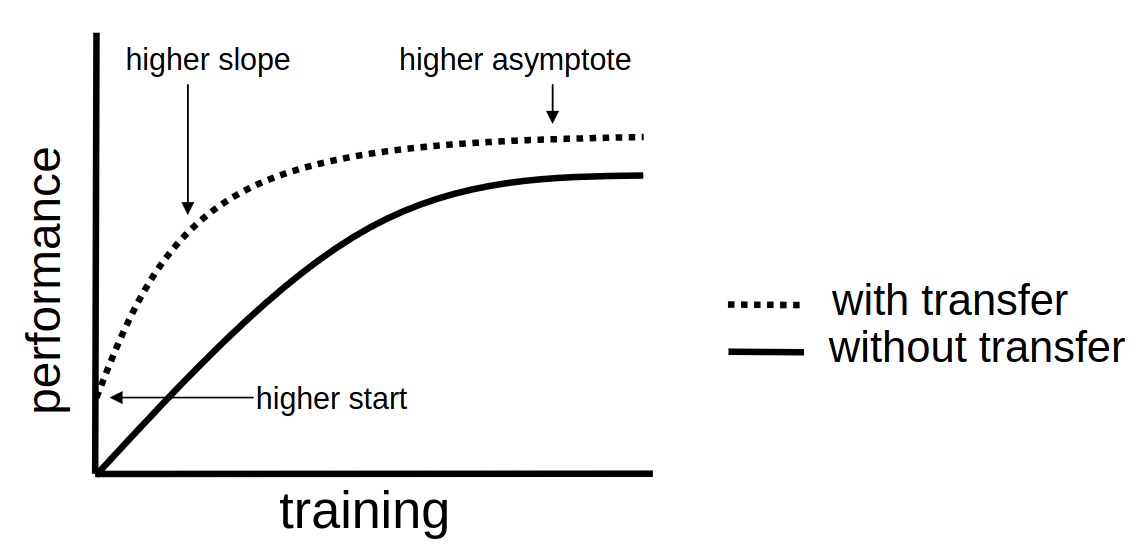
\includegraphics[width=0.7\linewidth]{images/performance.png}
              \caption{Figure taken from \cite{torrey-handbook} showing three ways in which transfer might improve learning}
              \label{fig:performance}
          \end{figure}


\end{itemize}

\subsection{Disadvantages}

\begin{itemize}
    \item Domain mismatch if the two models are trained on domains that are vastly different or with a different data distribution \cite{geeks-transfer-learning}.
    \item Overfitting `Transfer learning can lead to overfitting if the model is fine-tuned too much on the second task, as it may learn task-specific features that do not generalize well to new data.' \cite{geeks-transfer-learning}.
\end{itemize}

\subsection{General Approach}

This boils down to three questions: (1) What to transfer, (2) How to transfer, and (3) When to transfer.

Some knowledge may be common between different domains such that they may help improve performance for the target domain or task. When the source domain and target domain are not related to each other, brute-force transfer may be unsuccessful. In the worst case, it may even hurt the performance of learning in the target domain, a situation which is often referred to as negative transfer (see Section \ref{sec:negative-transfer}).

\subsubsection{Strategy}

\begin{enumerate}
    \item Obtain a pre-trained 'base' model. This model has been trained on extensive data and has identified general features and patterns relevant to numerous related jobs.
    \item Identify the transfer-layers. These capture generic information relevant to the new task as well as the previous one. These are 'frozen' in the final deliverable (see Figure \ref{fig:frozen-layers}) as we want to preserve the low-level learnt features. A layer is frozen or 'fixed' when it is no longer avaialble for training, hence the weights of these layers will not be avaialble for updates.
    \item Fine-tune and retrain the remaining layers. The goal is to preserve the knowledge from the pre-training while enabling the model to modify its parameters to better suit the demands of the current assignment. We can either
          \begin{itemize}
              \item freeze a few layers of the pre-trained model and train other layers on our new dataset for the new task
              \item or make a new model, but also take out some features from the layers in the pre-trained model and use them in a newly created model
          \end{itemize}
          The number of frozen layers depend on how much you want to inherit from the pre-trained model. If the networks are significantly different (i.e. use a human face detector to detect cars) selecting many layers for freezing will not only give low level features but also give high-level features like nose, eyes, etc which are useless for new dataset (car detection). Therefore, in this case you only copy the low level features \cite{geeks-transfer-learning}.

          \begin{lstlisting}[language=python] 
        
# freezing layers in python
for layer in base_model.layers: 
    layer.trainable = False

    \end{lstlisting}
\end{enumerate}

\begin{figure}[H]
    \centering
    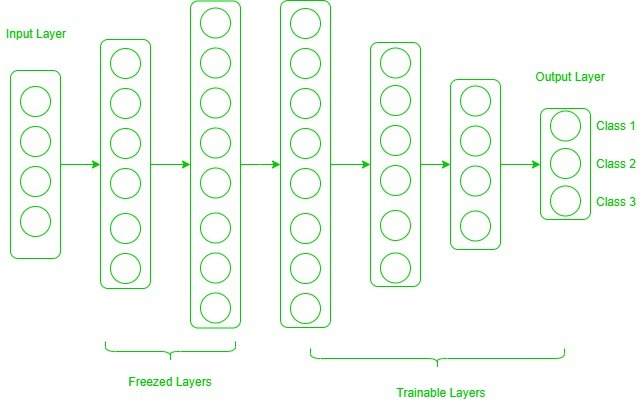
\includegraphics[width=0.7\linewidth]{images/Frozen-layers.jpg}
    \caption{Figure taken from \cite{geeks-transfer-learning} illustrating frozen and trainable layers from pre-trained and fine-tuned network.}
    \label{fig:frozen-layers}
\end{figure}

\subsection{Recommendations}

\begin{itemize}
    \item \textbf{The target dataset is small and similar to the base network dataset}: There may be an issue of overfitting because fine-tune the pre-trained network with the target dataset may not generalise to the global population. Also, there may be some changes in the number of classes in the target task; remove the fully connected layers from the end and add a new fully connected layer satisfying the number of new classes. Now, we freeze the rest of the model and only train newly added layers \cite{geeks-transfer-learning}.
    \item \textbf{The target dataset is small and different from the base network dataset}: Since the target dataset is different, using high-level features of the pre-trained model will not be useful. In such a case, remove most of the layers from the end in a pre-trained model, and add new layers a satisfying number of classes in a new dataset. This way we can use low-level features from the pre-trained model and train the rest of the layers to fit a new dataset. Sometimes, it is beneficial to train the entire network after adding a new layer at the end \cite{geeks-transfer-learning}.
    \item \textbf{Set the learning rate to be low}: It is essential to utilize a lower learning rate when compiling the new model because you are training a much larger model and want to readjust the pretrained weights. If not, your model may rapidly become overfit \cite{geeks-transfer-learning}. Furthermore, this is done for a low number of iterations for the same reasons \cite{deep-learning-book}.
    \item \textbf{Don't use stochastic gradient descent algorithms to the whole network}; it is much more efficient to send the new training data once through the fixed pre-trained network so as to evaluate the training inputs in the new representation. Iterative gradient-based optimization can then be applied just to the smaller network consisting of the final     layers.
\end{itemize}

\section{Avoiding Negative Transfer} \label{sec:negative-transfer}

If a transfer method actually decreases performance, then negative transfer has occurred. One of the major challenges in developing transfer methods is to produce positive transfer between appropriately related tasks while avoiding negative transfer between tasks that are less related \cite{torrey-handbook}.

\subsection{Fixes}

Reference \cite{torrey-handbook} contains a lot of useful sources regarding sources of different ideas surrounding transfer learning in different domains that might be extensible to a medical domain. This source was found through the source \cite{ gentle-introduction-to-transfer-learning}.

\subsubsection{Rejecting Bad Information}

The goal in this approach is to minimize the impact of bad information, so that the transfer performance is at least no worse than learning the target task without transfer. At the extreme end, an agent might disregard the transferred knowledge completely, but some methods also allow it to selectively reject parts and keep other parts \cite{torrey-handbook}.

\subsubsection{Choosing a subtask}

Eaton and DesJardins ``propose choosing from among candidate solutions to a source task rather than from among candidate source tasks. Their setting is multi-resolution learning, where a classification task is solved by an ensemble of models that vary in complexity. Low-resolution models are simple and coarse, while higher-resolution models are more complex and detailed'' \cite{torrey-handbook}.

\subsubsection{Modelling Task Similarity}

Given multiple candidate source tasks, it may be beneficial to use several or all of them rather than to choose just one.

``Ruckert and Kramer look at inductive transfer via kernel methods. They learn a meta-kernel that serves as a similarity function between tasks. Given this and a set of kernels that perform well in source tasks, they perform numerical optimization to construct a kernel for a target task. This approach determines the inductive bias in the target task (the kernel) by combining information from several source tasks whose relationships to the target are known'' \cite{torrey-handbook}.

\section{Transfer Learning Settings}

\begin{figure}[H]
    \centering
    \subfigure[Relationship between Traditional Machine Learning and Various Transfer Learning Settings]{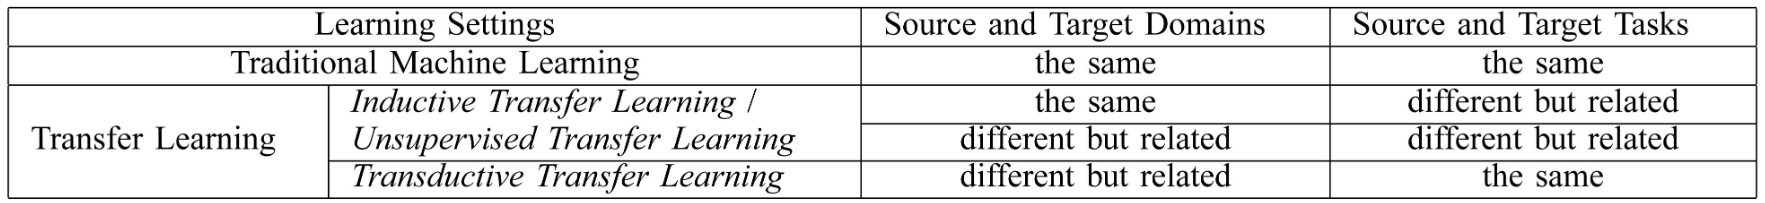
\includegraphics[width=\linewidth]{images/transfer-learning-settings.png}}

    \subfigure[Different Settings of Transfer Learning]{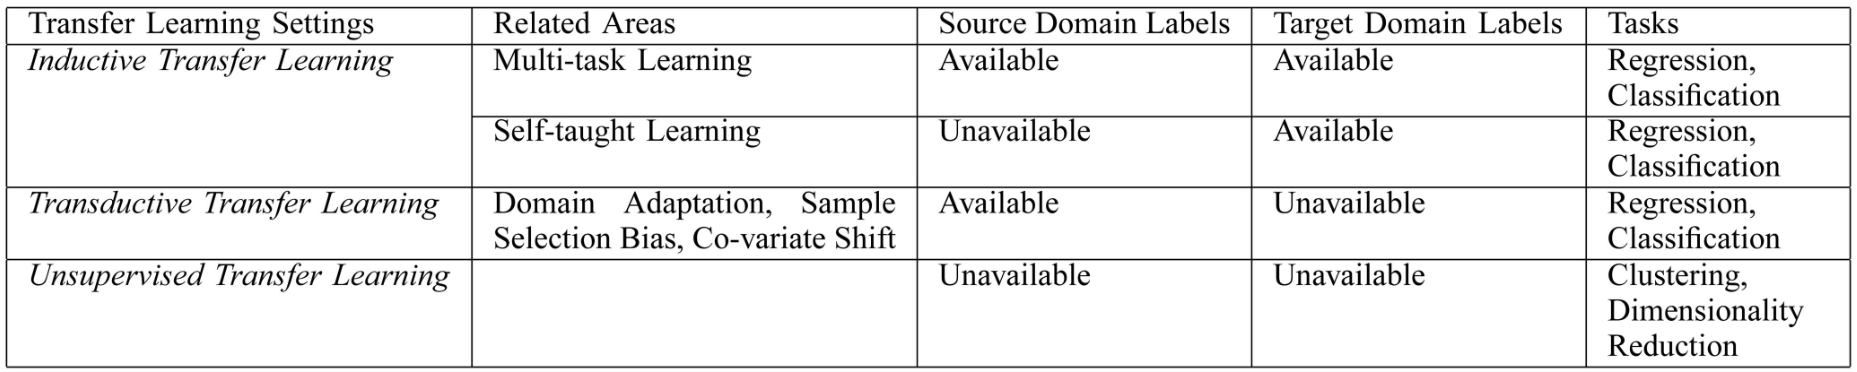
\includegraphics[width=\linewidth]{images/transfer-learning-settings-2.png}}

    \subfigure[An overview of different settings for transfer learning\label{fig:tree}]{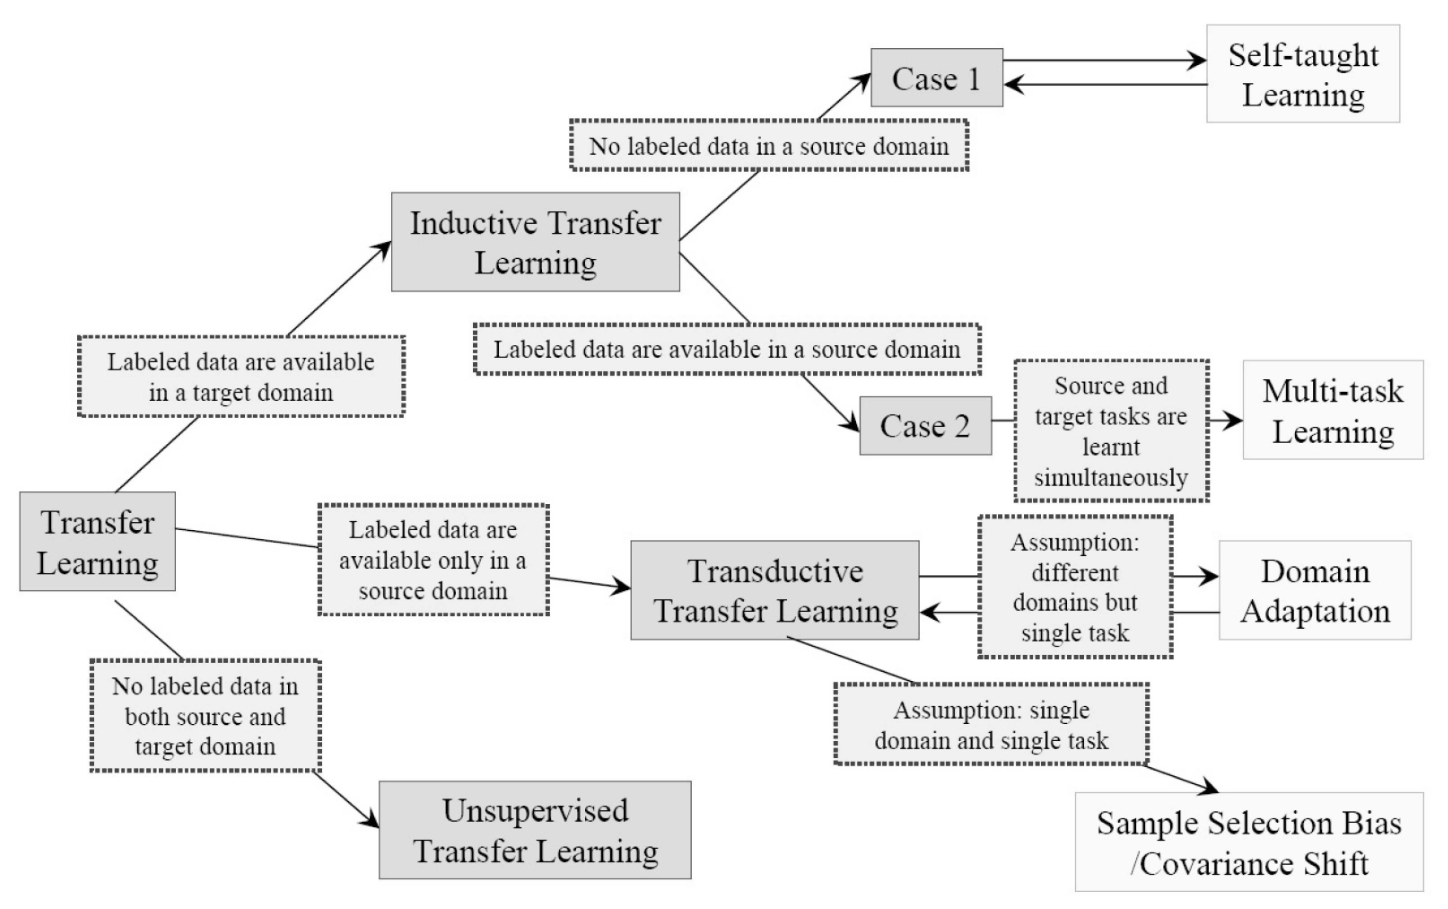
\includegraphics[width=\linewidth]{images/transfer-learning-tree.png}}
\end{figure}

\begin{figure}[H]
    \subfigure[Different Approaches to Transfer Learning]{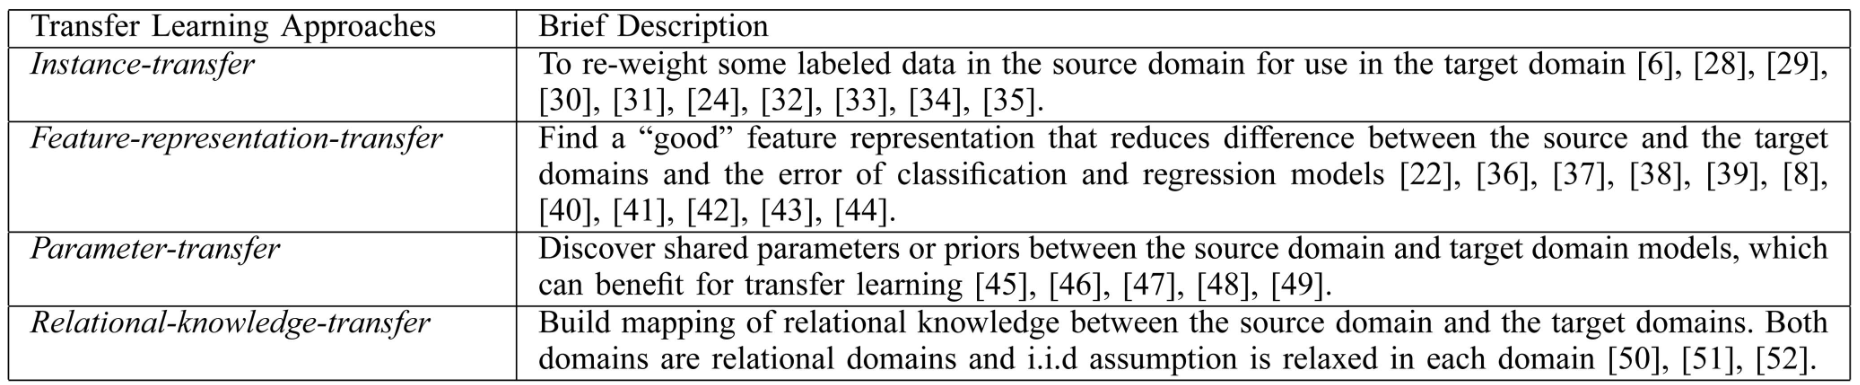
\includegraphics[width=\linewidth]{images/Different Approaches to Transfer Learning.png}}

    \subfigure[Different Approaches Used in Different Setings\label{fig:approaches}]{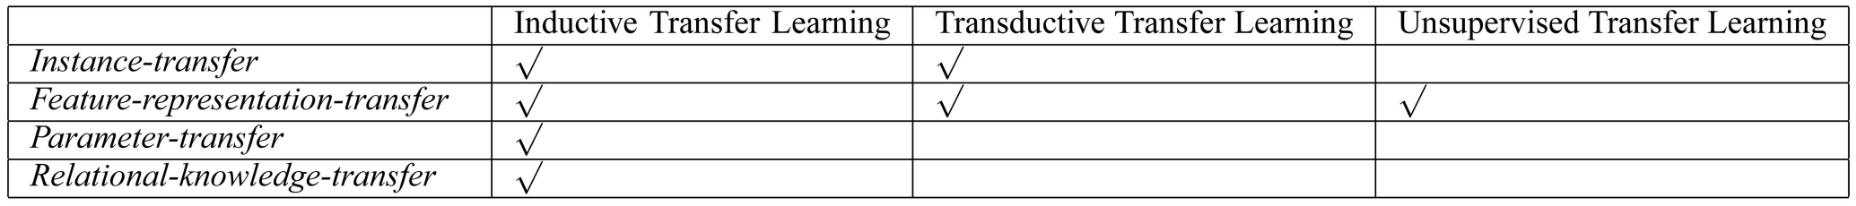
\includegraphics[width=\linewidth]{images/Different Approaches Used in Different Settings.png}}

    \caption{Taken from \cite{survey-on-transfer-learning}}
\end{figure}    

\subsection{Inductive Transfer Learning}

Relevant for our case is the branch from Figure \ref{fig:tree} is `Labeled data are avaialble in a target domain'. Therefore we lookup these cases only.

\subsection{Instance-transfer Approach}

From Figure \ref{fig:approaches} we have a source domain data which cannot be reused directly, however, there are certain parts of the data that can still be reused together with a few labeled data in the target domain. Note that there exist boosting algorithms TrAdaBoost (see \cite{transfer-learning-boosting} which details the algorithm for updating weight vectors).

\vspace{1em}

See further info at \cite{survey-on-transfer-learning}

\section{Sources of pre-trained models}

From \cite{gentle-introduction-to-transfer-learning} we have sources of pre-trained networks available at \href{https://github.com/BVLC/caffe/wiki/Model-Zoo}{Model-Zoo Github} as well as a \href{https://machinelearningmastery.com/how-to-use-transfer-learning-when-developing-convolutional-neural-network-models/}{walk-through}.

\printbibliography

\end{document}